\documentclass[12pt]{article}
\usepackage[utf8]{inputenc}
\usepackage[english]{babel}
\usepackage{natbib}
\usepackage{graphicx}
\usepackage{hyperref}
\usepackage{amsmath}
\usepackage{setspace}
\usepackage{geometry}
\usepackage{float}
\usepackage{authblk}
\usepackage[colorinlistoftodos]{todonotes}
\geometry{margin=1in}
\setstretch{1.2}

\title{\textbf{The Illusion of Optimality: Bias, Variance, and Informational Efficiency of Multi-Risk Assessments}}
\author[1]{Alexandre Dunant}
\author[1]{Stefano Terzi}

\affil[1]{EURAC Research, Bolzano, Italy}


\begin{document}
\maketitle

\begin{abstract}
Efforts to integrate multiple hazards, exposure and vulnerabilities into coherent risk frameworks have advanced over the past three decades, yet the field continues to lack operationalisable metrics to assess whether increasing model complexity has improved predictive or decision-making efficiency. This paper argues that the bias–variance tradeoff, originally from statistical learning theory, can serve as an analytical lens to interpret this trajectory and to ask whether the field's growing complexity reflects genuine progress or an "illusion of optimality". Without explicit measures of informational efficiency, risk integration could become performative rather than functional. We acknowledge that the path toward optimality must be reconciled with the actionability required by practitioners, and that once social components become central to an assessment, what counts as ``optimal'' is no longer technically determined but becomes relational, context-dependent, and contested. The paper therefore does not prescribe a universal optimum, but uses the bias--variance continuum as a diagnostic lens to ask whether current integration efforts move the field toward or away from informational efficiency---however that efficiency is ultimately defined

\end{abstract}

 \section{Introduction}
The bias--variance framework provides a pragmatic analytical argument for a long-standing challenge in risk science: determining when integration enhances understanding and when it merely amplifies uncertainty. Initially developed in machine learning, the concept describes the tradeoff between underfitting (high bias) and overfitting (high variance). Building on \citet{Dunant2021}, who first applied this framework as an analytical argument to multi-hazard risk assessments, this paper extends the analysis in three directions: (i) a three-phase historical mapping of the field's trajectory onto the bias--variance continuum, (ii) the introduction of \textit{informational efficiency} as a core evaluative concept, and (iii) a diagnosis of the ``illusion of optimality''---the risk that increasing complexity is mistaken for progress in the absence of shared efficiency metrics.

We specifically refer throughout to ``multi-risk'' frameworks as defined by \citet{zschau20172}: integrated systems that account for complex interactions among multiple hazards, exposed assets, and societal vulnerabilities---as distinct from simpler multi-hazard approaches that consider co-occurrence without systemic interdependencies. It is important to specify that regardless of the terminological scope---whether strictly multi-hazard (physical processes), multi-hazard risk (asset exposure), or multi-risk (systemic societal vulnerability)---the informational challenge is identical. Each step up this hierarchy introduces new parameters, thereby increasing the risk of variance (overfitting) if the underlying process understanding does not scale at the same rate as the model's complexity.

As \citet{Dunant2021} highlighted, single-hazard models in multi-hazard environments exhibit high bias, while overly complex multi-risk models show high variance without proportional gains in predictive accuracy (Figure~\ref{fig:BV-figure}). However, this framework has remained largely theoretical. The field lacks operationalisable metrics---quantitative where measurable, qualitative where not---to situate itself within this landscape; whether it sits near an optimal balance or drifts toward inefficiency remains unknown. This paper argues that \textit{informational efficiency}---the capacity to convert increased model complexity into proportional gains in uncertainty-aware, decision-relevant outputs---should become a core evaluative dimension of multi-risk science. The concept draws on decision theory \citep{Horvitz1995DisplayOIA}, information theory \citep{shannon1948mathematical, varley2025information}, and risk communication research \citep{Klinke2002ANAB}. We acknowledge, however, that explicitly measuring efficiency may not in itself dissolve the illusion of optimality, particularly when social systems resist the very notion of a clear-cut and universal optimum. The argument is therefore not that better metrics will solve the problem, but that without any shared language of efficiency, the field cannot even diagnose where it stands.

\section{Conceptual Framework}
The bias--variance framework is used here, as in \citet{Dunant2021}, as a conceptual heuristic---not as a literal statistical mapping. In statistical learning theory, bias and variance are mathematically decomposable components of prediction error; in multi-risk science, they are not. The analogy is therefore diagnostic rather than quantitative: it provides a vocabulary for asking whether a given integration effort errs toward oversimplification (high bias) or toward unmanageable complexity (high variance), without implying that formal decomposition is possible.

This lens applies beyond physical models. In participative exercises, the pursuit of comprehensive social integration may introduce redundancy, conflicting inputs, or epistemic noise---the accumulation of incommensurable knowledge claims from diverse disciplinary and stakeholder perspectives that reduce the clarity of causal inference and impede actionable synthesis \citep{Schlter2024NavigatingCRA, rusca_water_2026}---thereby diminishing informational efficiency without commensurate gains in decision relevance. This complexity also directly undermines interpretability: if practitioners cannot trace the causal logic amidst the noise of competing narratives, they cannot assume the professional responsibility required to translate assessments into action \citep{pereira2024integrating}.

In this context, the pursuit of ``multi-risk'' optimality must account for bounded rationality \citep{Simon1956, Simon1947} and acknowledge the absence of ``unlimited resources of time, information, and computational might'' \citep{gigerenzer2020bounded}. Analogous to the ``efficiency--resilience'' tradeoff \citep{Hynes2020}, hyper-integration (low bias) could produce an ``integration--resilience tradeoff'', where noise overtakes the capacity for action.

\begin{figure}[H]
    \centering
    \resizebox{\linewidth}{!}{% Input-only TikZ fragment.
% Main-document preamble requirements:
% \usepackage{graphicx,float,tikz}
% \usetikzlibrary{positioning,arrows.meta,calc}

\definecolor{biasred}{RGB}{175,35,35}
\definecolor{varteal}{RGB}{25,145,150}
\definecolor{totalblack}{RGB}{20,20,20}
\definecolor{boxbg}{RGB}{252,252,252}
\definecolor{ph1}{RGB}{170,35,35}
\definecolor{ph2}{RGB}{45,110,55}
\definecolor{ph3}{RGB}{30,95,165}

\begin{tikzpicture}[font=\normalsize]

% ---------- geometry ----------
\def\xmax{7.2}
\def\ymax{5.3}
\def\xopt{4.13}
\def\yopt{0.85}
\def\timex{7.95}
\def\boxx{8.75}

% ---------- styles ----------
\tikzset{
  ax/.style={-{Latex[length=3mm,width=2.3mm]}, line width=1.3pt, totalblack},
  cv/.style={line width=2.1pt, samples=220, domain=0.02:9.5},
  lead/.style={line width=0.6pt, opacity=0.85},
  phasebox/.style={draw=#1, fill=boxbg, rounded corners=5pt, line width=1pt,
                   text width=5.15cm, inner xsep=6pt, inner ysep=5pt, % was 6pt
                   align=left, font=\small},
}

% Shift the complete landscape left; the timeline and phase boxes stay fixed.
\begin{scope}[xshift=-5mm]

% ---------- axes ----------
\draw[ax] (-0.2,0) -- (\xmax+0.25,0);
\draw[ax] (0,-0.2) -- (0,\ymax+0.25);
\node[font=\large\bfseries, totalblack, anchor=north west]
      at (5.10,-0.24) {Complexity};
\node[font=\large\bfseries, totalblack, rotate=90]
      at (-0.58,{0.46*\ymax}) {Error};

% ---------- curves ----------
\begin{scope}
  \clip (0,0) rectangle (\xmax,\ymax);
  \draw[cv,biasred]
    plot (\x,{5*exp(-0.6*\x)+0.07});
  \draw[cv,varteal]
    plot (\x,{0.02*exp(0.7*\x)});
  \draw[cv,totalblack,line width=2.4pt]
    plot (\x,{5*exp(-0.6*\x)+0.02*exp(0.7*\x)+0.07});
\end{scope}

% ---------- optimum ----------
\draw[totalblack!45, dashed, line width=1pt]
  (\xopt,0.08) -- (\xopt,\ymax-0.35);
\filldraw[fill=white, draw=totalblack, line width=1pt]
  (\xopt,0) circle (0.14);
\fill[totalblack] (\xopt,\yopt) circle (0.07);
\node[font=\small\bfseries, totalblack!75, anchor=north east]
  at (\xopt-0.12,-0.25) {Optimum};
\node[font=\footnotesize\itshape, totalblack!60, anchor=north,
      align=center, text width=4.8cm]
  at (\xopt,-0.77)
  {Position of current practice relative to this optimum unknown};

% ---------- curve labels ----------
\node[biasred, font=\normalsize\bfseries, anchor=west]
  at (1.00,0.80) {Bias$^2$};
\draw[lead,biasred] (2.18,0.93) -- (2.53,1.12);
\fill[biasred] (2.55,1.15) circle (0.05);

\node[varteal, font=\normalsize\bfseries, anchor=west]
  at (5.35,0.55) {Variance};
\draw[lead,varteal] (5.95,0.78) -- (6.17,1.46);
\fill[varteal] (6.20,1.53) circle (0.05);

\node[totalblack, font=\normalsize\bfseries, anchor=east]
  at (3.90,3.00) {Total Error};
\draw[lead,totalblack] (3.45,2.80) -- (3.07,1.11);
\fill[totalblack] (3.05,1.04) circle (0.05);

% ---------- unknown current position ----------
% The two free-floating "?" glyphs are gone: they read as stray characters.
% The "position undetermined" statement now lives in the note under the axis,
% in the Phase III box, and in the caption. If you want a visual hook back,
% use this self-explanatory badge instead of bare question marks:
% \node[draw=ph3!50, dashed, thick, rounded corners=4pt, align=center,
%       inner sep=4pt, text=ph3!75, font=\large\bfseries]
%   at (5.90,4.20) {?\\[-1pt]\scriptsize\normalfont\itshape current practice};

\end{scope}

% ---------- phase boxes (tighter column: 6 mm gaps, 5 pt y-sep) ----------
\node[phasebox=ph1, anchor=north west] (box1) at (\boxx,\ymax)
  {\textcolor{ph1}{\large\bfseries Phase I}\hspace{5pt}%
   \textcolor{ph1}{\footnotesize Pre-2005}\\[4pt]
   Siloed models\\[1pt]
   Disciplinary silos};

\node[phasebox=ph2, below=6mm of box1] (box2)
  {\textcolor{ph2}{\large\bfseries Phase II}\hspace{5pt}%
   \textcolor{ph2}{\footnotesize 2005--?}\\[4pt]
   Institutional integration\\[1pt]
   Participatory approaches};

\node[phasebox=ph3, below=6mm of box2] (box3)
  {\textcolor{ph3}{\large\bfseries Phase III}\hspace{5pt}%
   \textcolor{ph3}{\footnotesize ? (unverified)}\\[4pt]
   ``Model of everything''\\[1pt]
   Position on landscape \textbf{undetermined}};

\draw[-{Latex[length=2.2mm,width=1.8mm]}, black!35, line width=0.9pt]
  (box1) -- (box2);
\draw[-{Latex[length=2.2mm,width=1.8mm]}, black!35, line width=0.9pt]
  (box2) -- (box3);

% ---------- temporal separator (auto-centred on the box column) ----------
\coordinate (timelinetop) at (\timex,\ymax);
\coordinate (timelinebottom) at (timelinetop |- box3.south);
\draw[-{Latex[length=3mm,width=2.3mm]}, black!40, line width=1.2pt]
  (timelinetop) -- (timelinebottom);
\node[font=\small\itshape, black!55, rotate=90, anchor=center]
  at ([xshift=-4mm]$(timelinetop)!0.5!(timelinebottom)$)
  {Temporal evolution};

\end{tikzpicture}}
    \caption{Conceptual framing of the bias--variance landscape for multi-risk assessments.}
    \label{fig:BV-figure}
\end{figure}

The following sections categorise the evolution of multi-risk science into three chronological phases, mapping the field's trajectory onto the bias--variance continuum \citep{Dunant2021}. This framing illustrates the transition from the high-bias simplicity of siloed origins to the high-variance complexity of modern hyper-integration, allowing for a critical evaluation of whether current integration efforts achieve functional efficiency or merely drift toward an ``illusion of optimality''.

\section{Phase I: Siloed Origins and Emerging Integration Mandates (before 2005)}
The first attempts to formalize multi-hazard assessment emerged alongside early international frameworks promoting integrated disaster management. On the science side, the volcanology community provided significant early precedents in this regard, as volcanic crises inherently involve the interaction of multiple simultaneous hazards like ashfall,
lahars, and seismic activity \citep{tilling1989volcanic, blong1996volcanic}.

\begin{figure}
    \centering
    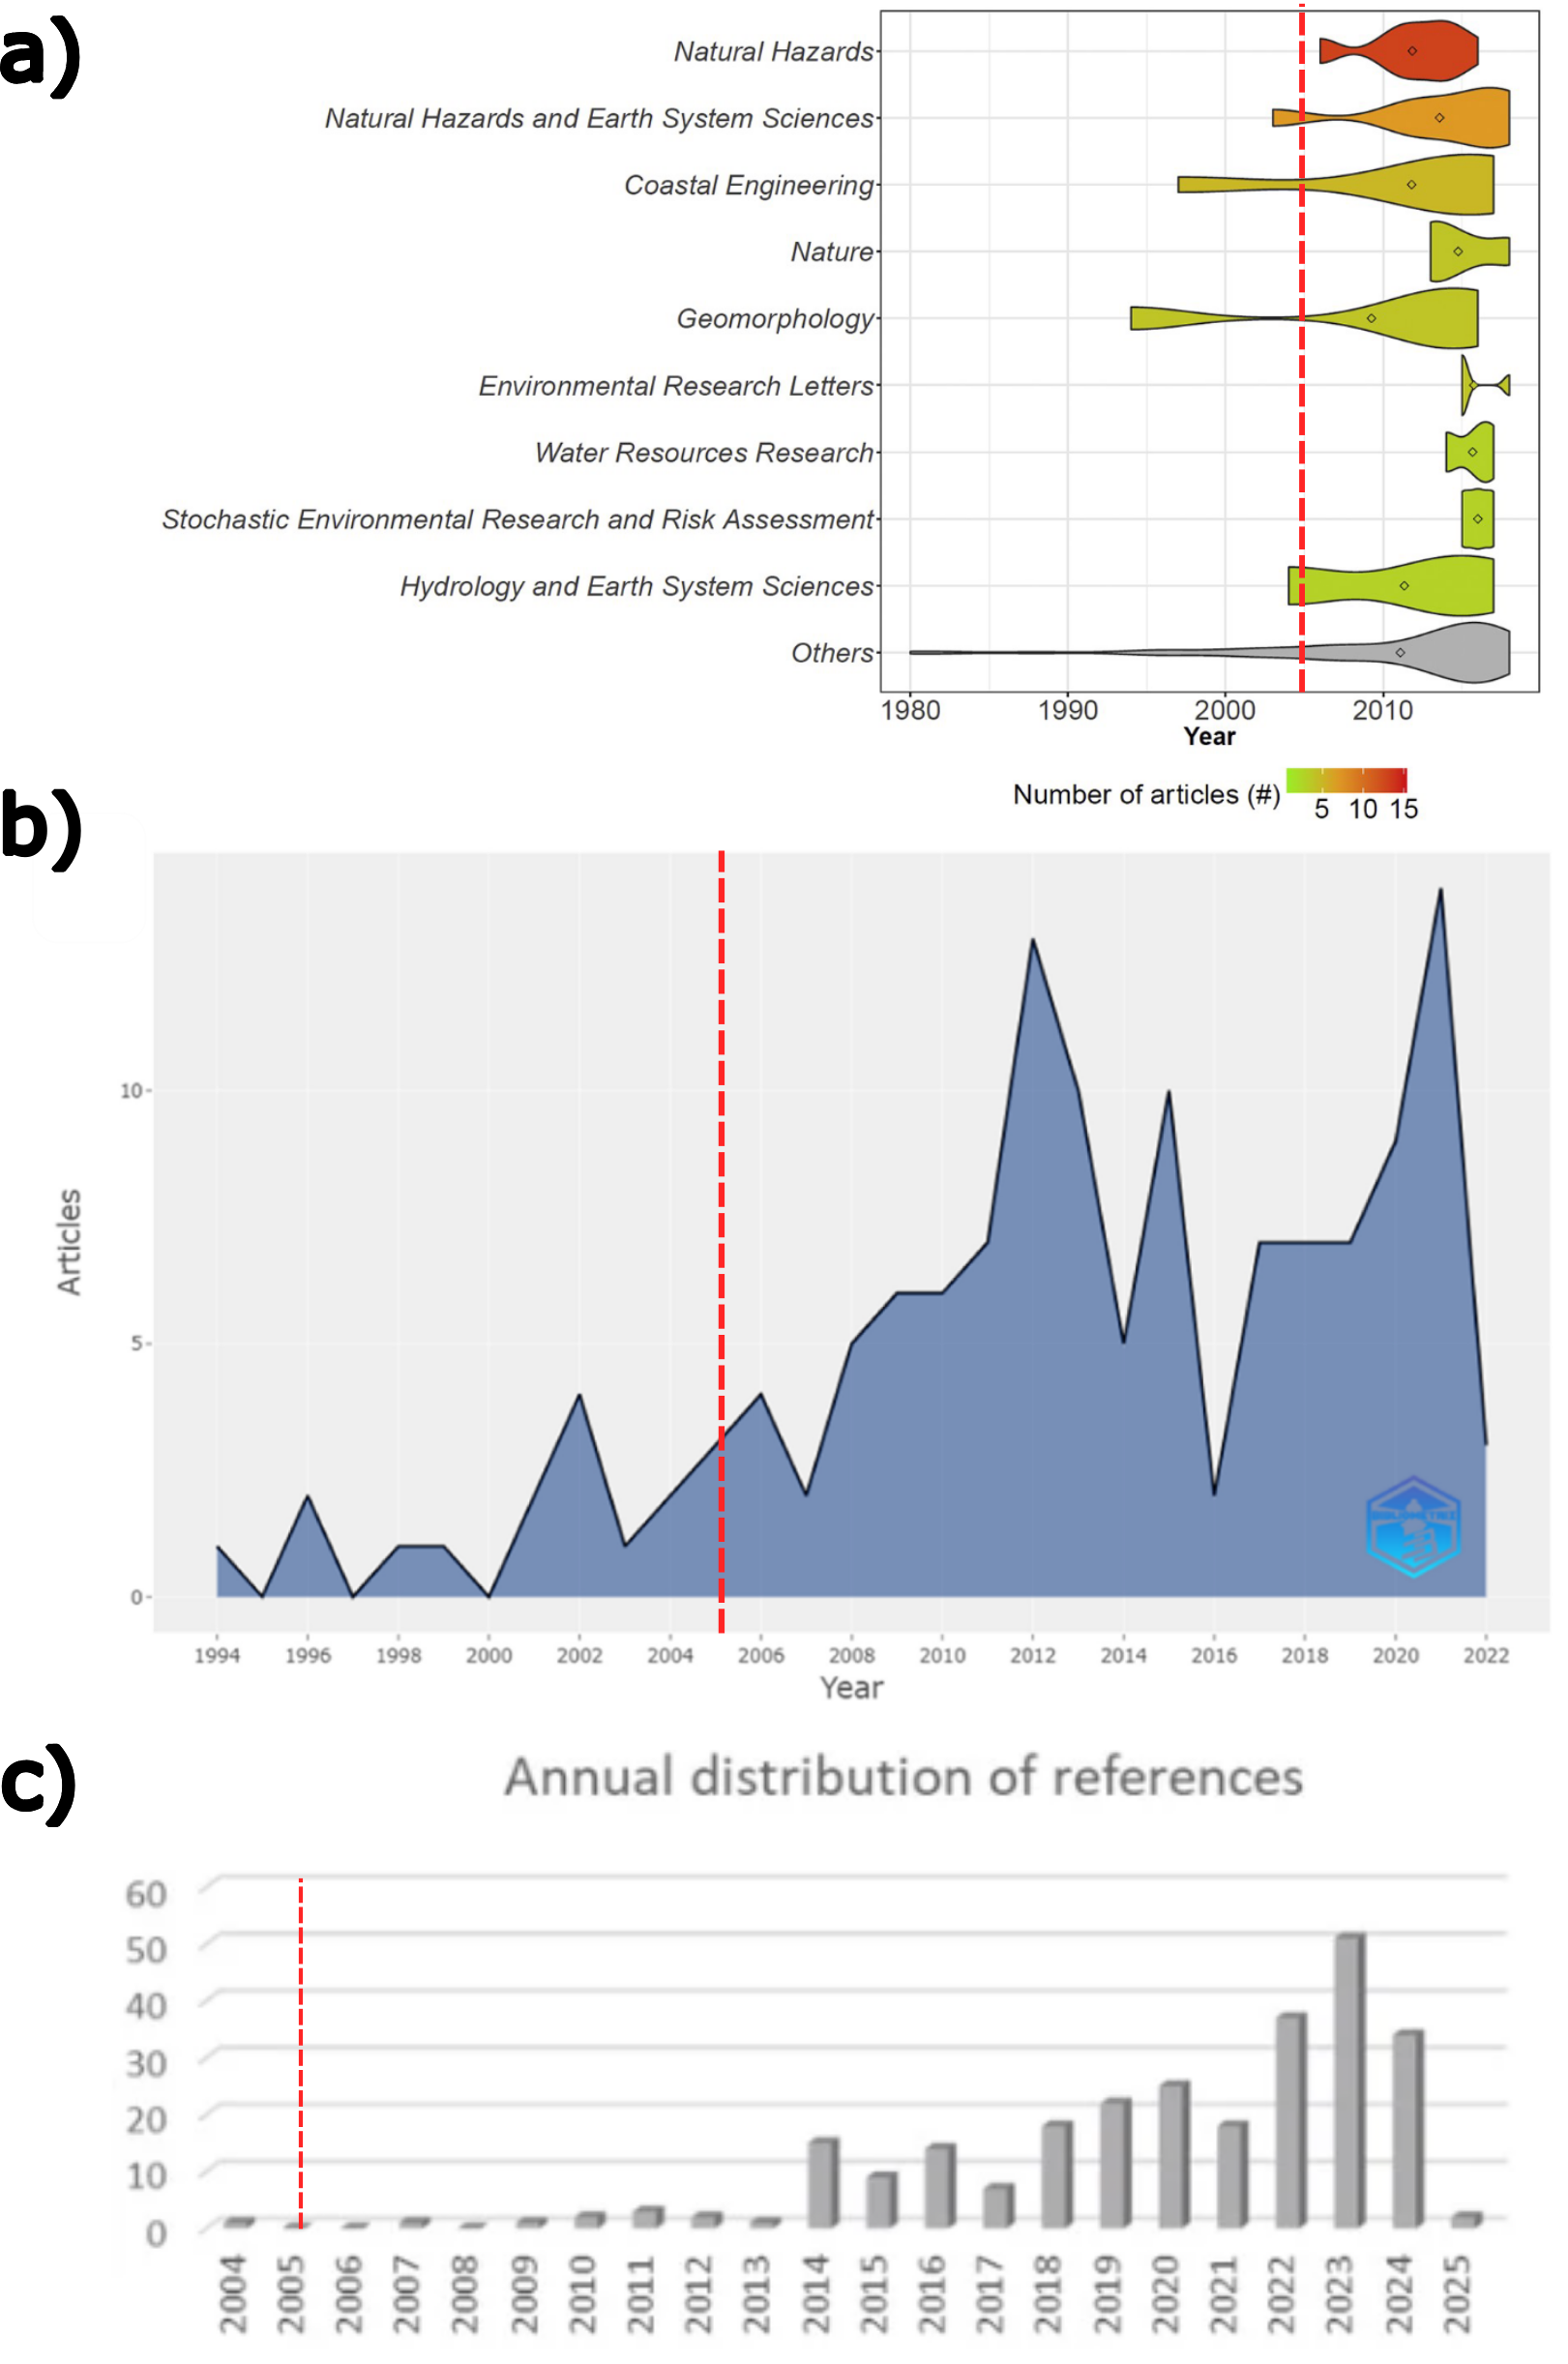
\includegraphics[width=0.75\linewidth]{bibliom_multihazard.png}
    \caption{Bibliometric analysis of multihazard and multirisk litterature by a) \cite{Tilloy2019} b) \cite{Owolabi2023} and c) \cite{grandjean2025bibliographic}, with the red dotted line highlighting the year 2005.}
    \label{fig:placeholder}
\end{figure}

The principles of sustainable development outlined in \textit{Agenda 21} \citep{Agenda21_1992} and later reinforced by the Johannesburg Plan \citep{UN2002} and the Hyogo Framework for Action \citep{HyogoFramework2005} established the groundwork for multi-hazard thinking.  

During this phase, risk assessments remained largely disciplinary, emphasizing individual hazards such as floods, earthquakes, or landslides. Studies like \citet{Middelmann2000} and \citet{granger1999community} in Australia exemplified early local-scale multi-hazard assessments. At this stage most models exhibited high bias: simplified assumptions and a focus on single-event probabilities regardless if they happened in a multi-hazard environment. 

The absence of uncertainty quantification and the reliance on heuristic matrices led to low informational efficiency models were interpretable but detached from cascading dynamics and long-term systemic risks. Conceptual work by \citet{Marzocchi2009} and \citet{kappes_challenges_2012} articulated the need for frameworks addressing multi-hazard and multi-risk interactions as single-hazard approaches in multi-hazard environments are inherently biased toward specific features, missing critical interdependencies and paved the way to "Phase II" presented in the following paragraph.

\section{Phase II: Institutional Integration and the Illusion of Optimality (2005–?)}

Following the Hyogo Framework, institutional momentum accelerated the integration of multiple hazards. The Sendai Framework \citep{SendaiFramework2015} later reaffirmed this mandate, emphasizing "all-of-society" and "systemic" approaches. These international mandates, by prioritizing 'holistic' and 'all-hazard' frameworks, effectively incentivized the creation of 'super models'—comprehensive systems designed to map every interaction. The transition from single-hazard to systemic multi-risk assessments is, in part, driven by what \citet{zschau20172, hochrainer2024managing} identifies as the twin challenges of risk globalisation and climate change. Globalisation has rendered risks interdependent through cross-linked critical infrastructure and global supply chains, while climate change increases the frequency and spatial distribution of extreme events \citep{seneviratne2021weather}. These drivers create "high-risk dynamics" that require capturing various interactions \citep{pescaroli2018understanding}, simultaneously stimulating the bias-tradeoff variance dilemma highlighted herein.

Research during this phase reduced bias by linking hazard chains, introducing Bayesian networks, and incorporating network-based or spatio–temporal frameworks (\citealt{Tilloy2019}; \citealt{DeAngeli2022}; \citealt{Terzi2019}; \citealt{dunant2021multihazards} \citealt{dunant2025impacts}). These efforts represented a major step toward a unified understanding of cascading effects and feedback loops. At this stage, multi-hazard adoption induced a rise in variance of the risk models.

Yet the apparent convergence toward optimality was deceptive. Several reviews show that integration often increased conceptual overlap but still struggle to translate complexity into actionable indicators \citep{Owolabi2023, laino2024scientometric, hochrainer2024managing, scolobig2017mainstreaming}. The field seems to achieve visibility but not necessarily efficiency - defined here as the ability to convert increased model complexity into proportional gains in decision relevance. The illusion of optimality persisted not simply because standardized metrics were absent, but because the very notion of what constitutes an informational gain was never made explicit: whether efficiency should be measured in terms of improved risk communication, facilitated action, or deeper process understanding remained unarticulated. This ambiguity---not merely a technical gap---is what could allow increasing complexity to be mistaken for progress. \citet{Dunant2021}'s warning that as model complexity increases, the risk of "overfitting" escalates, potentially impairing the practical precision of multi-hazard outputs, is even more prevalent today as the tools, for large scale computation and collaboration become, more accessible \citep{mack2011fifty}.

\section{Phase III: Rising Complexity and the Unquantified Present (?)}
The authors believe the field (i.e. multi-hazard, multi-risk) stands at a crossroads today. Advances in computational modelling, remote sensing, and machine learning have enabled "hyper-integrated" frameworks spanning climate, geophysical, and social domains (\citealt{Ferrario2025}; \citealt{MYRIAD2022}; \citealt{lundstrom2022moore}). However, these systems risk overfitting: absorbing massive input data into interconnected systems without tangible measurable improvement in output quality or decision usability. 

As demonstrated by recent assessments of European transboundary risk management, the primary hurdle to operationalizing multi-risk science is not a lack of model complexity, but a lack of fundamental harmonization in metrics and data structures across borders \citep{polese2024multi}. While scientific "super-models" attempt to simulate complex hazard interactions, practitioners are often still restricted by a "fragmented data landscape" and a lack of common vulnerability classes, which makes the outputs of highly integrated models difficult to compare or legally validate in an operational context \citep{polese2024multi}. Furthermore, as \citet{kalogiannidis2024analyzing} highlight, the effectiveness of disaster management in Europe is more significantly hindered by administrative and legislative obstacles—such as the lack of standardized protocols—than by a lack of computational integration. This suggests that the "illusion of optimality" in complex modelling fails to account for the "social reality" of the legal and administrative constraints within which Civil Protection agencies must operate.

Informational efficiency—defined here as the ratio between usable, uncertainty-aware outputs and the complexity of model inputs—remains largely untracked. Without such metrics, integration can drift into epistemic opacity, where uncertainty and redundancy coexist. As \citet{dunant2021multihazards} emphasized, finding a "healthy medium between accuracy (bias) and precision (variance)" requires quantifying the relationship between model complexity, risk and action.

Future progress depends on being honest about what kind of progress is being made.The objectives of \textit{scientific progress} (advancing process understanding) and \textit{operational progress} (supporting defensible decisions) are not opposed, but they optimise differently and require different standards of evaluation. Conflating them risks producing the ``Mushy Middle'' \citep{stonehouse2007competitive}: work that achieves neither genuine process insight nor novel operational application---sophisticated enough to appear rigorous, tractable enough to appear useful, but evaluated against neither standard. For the researcher, the relevant question is therefore not whether a model is complex, but whether its complexity resolves a specific gap in process understanding that simpler models cannot. For the practitioner, the question is whether it narrows the range of defensible decisions under uncertainty in a way that is institutionally actionable \citep{polese2024multi}.In both cases, the threshold for ``good enough'' is as much social and institutional as it is technical---it depends on who will use the output, under what constraints, and toward what decision \citep{HangerKopp2022, Simon1956}.
What the field currently lacks might not be more integration, but an explicit, shared account of these thresholds. Without it, efficiency claims remain unverifiable, complexity continues to be equated with progress, and the illusion of optimality persists \citep{scolobig2017mainstreaming, kalogiannidis2024analyzing}.

\section{Conclusion: Toward Quantifiable Efficiency in Multi-Risk Science}
The history of multi-risk assessment reflects oscillations between bias and variance rather than a smooth path to optimality. The current landscape demonstrates that complexity alone does not equate to progress. This paper, building on the foundational bias-variance perspective introduced by \citet{Dunant2021}, calls for a clear research intent and an emphasize toward tracking, an often sidelined, informational efficiency: the systematic evolution of how uncertainty, interpretability and usability with integration. The bias–variance framework is not an end in itself, but an analytical argument for a pragmatic requirement—the need to assess where we stand. Establishing shared metrics for uncertainty and informational efficiency is now essential for ensuring that the evolution of multi-risk modelling remains both rigorous and actionable in the midst of globally connected challenges.

\section*{Acknowledgements}

\section*{Competing Interests}
The author declares no competing interests.

\bibliographystyle{apalike}
\bibliography{references}

\end{document}
